%%%%%%%%%%%%
%% Please rename this main.tex file and the output PDF to
%% [lastname_firstname_graduationyear]
%% before submission.
%%%%%%%%%%%%

\documentclass[12pt]{caltech_thesis}
\usepackage[hyphens]{url}
\usepackage{lipsum}
\usepackage{amsmath}
\usepackage{graphicx}
\usepackage{needspace}
\usepackage{todonotes}
\usepackage{subcaption}

%% Tentative: newtx for better-looking Times
\usepackage[utf8]{inputenc}
\usepackage[T1]{fontenc}
\usepackage{newtxtext,newtxmath}

% Must use biblatex to produce the Published Contents and Contributions, per-chapter bibliography (if desired), etc.
\usepackage[
    backend=biber,natbib,
    % IMPORTANT: load a style suitable for your discipline
    style=authoryear
]{biblatex}

% Name of your .bib file(s)
\addbibresource{example.bib}
\addbibresource{ownpubs.bib}

\begin{document}

% Do remember to remove the square bracket!
\title{A Swampland Constraint on Gravitational Collapse}
\author{Himanshu Chaudhary}

\degreeaward{Master of Science, Physics}                 % Degree to be awarded
\university{Indian Institute of Science}    % Institution name
\address{Bangalore, India}                     % Institution address
\unilogo{images/iisc_logo.png}                                 % Institution logo
\copyyear{2020}  % Year (of graduation) on diploma
\defenddate{1 July 2020}          % Date of defense

\orcid{[Author ORCID]}

%% IMPORTANT: Select ONE of the rights statement below.
% \rightsstatement{All rights reserved\todo[size=\footnotesize]{Choose one from the choices in the source code!! And delete this \texttt{todo} when you're done that. :-)}}
% \rightsstatement{All rights reserved except where otherwise noted}
% \rightsstatement{Some rights reserved. This thesis is distributed under a [name license, e.g., ``Creative Commons Attribution-NonCommercial-ShareAlike License'']}

%%  If you'd like to remove the Caltech logo from your title page, simply remove the "[logo]" text from the maketitle command
\maketitle[logo]
% \maketitle

\begin{acknowledgements}
   I would like to thank my advisor Professor Chethan Krishnan for his guidance and constant encouragement. His insights about the problem helped me in avoiding a lot of pitfalls and wasted effort, allowing me to focus on the most important aspects of the problem. I would also like to thank Prof. Jun-Qi Guo for answering a lot of questions about the numerical parts of the problem.

   I would also like to thank my family for their continuous support and providing a mental sanctuary away from all the pressure that comes with academia.
   Finally, I would like to thank my friends and batch-mates for all the fruitful discussion that we had about the project and other courses.
\end{acknowledgements}

\begin{abstract}
   Gravitational collapse of a scalar field is a well studied phenomenon but, most of these studies are focussed on studying the field behavior close to criticality and its implications. In this thesis we revisit the problem of critical collapse but this time in context of swampland bounds. It has been speculated that a classical solution where the scalar fields move by an $O(1)$ range (in Plank units) signals the breakdown of Effective Field Theory, also known as the Swampland field range bound. In this thesis we show that during the gravitational collapse the scalar field moves by an $O(1)$ and discuss its implications in the context of the swampland field range bound.
\end{abstract}

%% Uncomment the `iknowhattodo' option to dismiss the instruction in the PDF.
% \begin{publishedcontent}%[iknowwhattodo]
%    % List your publications and contributions here.
%    \nocite{Cahn:etal:2015,Cahn:etal:2016}
% \end{publishedcontent}

\tableofcontents
\listoffigures
\listoftables
% \printnomenclature

\mainmatter


% \chapter{Guide}
Start off all chapters with \verb|chapter|. \index{chapter!numbered} \verb|\extrachapter| will give you an unnumbered chapter that's added to the Table of Contents. \index{chapter!unnumbered}

Here's an example of a citation \citep{GMP81}. Here's another \citep{PP98}. These will appear in the big bibliography at the end of the thesis.
\index{bibliography}


You can define nomenclatures \index{nomenclature} as you talk about key terms in your thesis. So what's a galaxy? \nomenclature{Galaxy}{A system of stars independent from all other systems}


\section{This is a Section}
\lipsum[1-2]

\begin{figure}[hbt!]
    \centering
    \includegraphics[width=.3\textwidth]{images/caltech.png}
    \caption{This is a figure}\label{fig:logo}
    \index{figures}
\end{figure}

\subsection{This is a subsection}

\begin{table}[hbt!]
    \centering
    \begin{tabular}{ll}
        \hline
        Area  & Count \\
        \hline
        North & 100   \\
        South & 200   \\
        East  & 80    \\
        West  & 140   \\
        \hline
    \end{tabular}
    \caption{This is a table}\label{tab:sample}
    \index{tables}
\end{table}

\lipsum[3] \nomenclature{Asteroid}{A very small planet ranging from 1,000 km to less than one km in diameter. Asteroids are found commonly around other larger planets}

\lipsum[4-5]

Here's an endnote.\endnote{Endnotes are notes that you can use to explain text in a document.}

\section{This is Another Section}
\lipsum[6-7]

\chapter{This is the Second Chapter}
\begin{refsection}
    If you'd like to have separate bibliographies at the end of each chapter, put a \verb|refsection| around the material of each chapter, then cite as usual -- e.g.~\citep{GMP81,Ful83}. Then do a \verb|\printbibliography| just before the \verb|refsection| ends. \index{bibliography!by chapter}

    \printbibliography[heading=subbibliography]
\end{refsection}


\chapter{This is the Third Chapter}

\publishedas{Cahn:etal:2015}

[You can have chapters that were published as part of your thesis. The text style of the body should be single column, as it was submitted to the publisher, not formatted as the publisher did.]

\chapter{This is the Fourth Chapter}
\chapter{This is the Fifth Chapter}
\chapter{This is the Sixth Chapter}
\chapter{This is the Seventh Chapter}
\chapter{This is the Eighth Chapter}



\chapter{Introduction}

The main focus of this study was to look at the gravitational collapse of a scalar field in the light of swampland distance conjecture. In the following sections we will briefly touch upon these topics and give suitable references for further explorations.

\section{Gravitational collapse of scalar fields}


Critical collapse of scalar fields in gravitation is a well studied phenomenon \citep{Gundlach:2007gc}, and there are many interesting results mostly based on the numerical simulations. Gravitational collapse and the numerical methods used to study it will be described in detail in a later chapter. Here we will just mention one result that will be required to put things that we are going to discuss into perspective.

Assume that the initial configuration of the scalar field is described by a function with n adjustable parameters that we are free to choose. Then for each one of those n parameters (that are not zero modes) there will be a corresponding threshold, crossing which will lead to the formation of a black hole.

For example, if the initial scalar field configuration is a gaussian shell with fixed mean and variance, then there will a critical value of the amplitude (let’s call it $A_0$ ) above which black hole formation will take place. Although, if we keep the amplitude (A) below $A_0$ then the scalar field will disperse to infinity. The same holds true for the mean and the variance.

An important thing that we will show via our simulations is that even if the initial value of the amplitude A and the critical value $A_0$ are both much smaller than 1, the scalar field will still move by $O(1)$ in supercritical cases. We will expand upon and give examples of this in later chapters.
For this chapter it is enough to remember that in general relativity scalar fields can move $O(1)$ distance in the scalar field space, starting from much smaller values.

\section{Swampland conditions}
Before we can appreciate what are swampland conditions we need to understand a little bit about effective field theories and the role that they play in Physics.

\subsection{Effective field theories}
Physical phenomenon occurs at various scales, sometimes we are only interested in the results at a particular scale. For example, if we are interested in the collision of two slow moving bodies then Newtonian mechanics is more than enough, we do not need to consider Relativistic mechanics. The scale of interest in this case is the kinetic energy (speed) of the bodies and for speeds much smaller than the speed of light we can consider Newtonian mechanics as an "effective theory" of Relativistic mechanics. When one usually talks about scales in an effective theory that scale is energy, here we used speed as our scale because the masses are fixed. Such theories in the context of QFT are known as "effective field theories".
% Roughly speaking we can set the parameters( which is mostly energy) much smaller and larger than the physical quantities we are interested in to zero and infinity respectively. After that, any effects due to these approximations can be included as small perturbations.



A prime example of an effective field theory is Fermi theory of weak interactions. It was phenomenologically constructed by Fermi as a modification to QED which accounted for the neutron decay. Now that we have the Standard model, we understand that the Fermi theory is an effective field theory valid for energy scales much smaller than the mass of W boson.

Effective theories are ubiquitous in Physics, whether it is for the ease of calculations (it is not an efficient use of time to track motion of a football using String Theory) or because they are a part of how Physics progresses (nobody could have constructed the Standard model lagrangian without the insights gained from all the effective field theories).
If we have a more "complete" theory, then it is a comparatively easy matter to generate effective theories as per our needs. At this point one can ask a question, can all field theories be extended into more general and complete theories?
The exact question that we are interested in is what kind of effective field theories can be completed into quantum gravity in the high energy or UV regime? This is the question that swampland conditions try to answer.


\subsection{The landscape and the swampland}
A lot of low energy effective field theories, each corresponding to a different vacuum, can be constructed from the string theory. The collection of such effective field theories constructed from the string theory is called the landscape. At the same time, there are a lot of other potentially complete low energy theories that when coupled to gravity lead to inconsistencies, the collection of all such theories is called the swampland.


% \begin{figure}[hbt!]
%     \centering
%     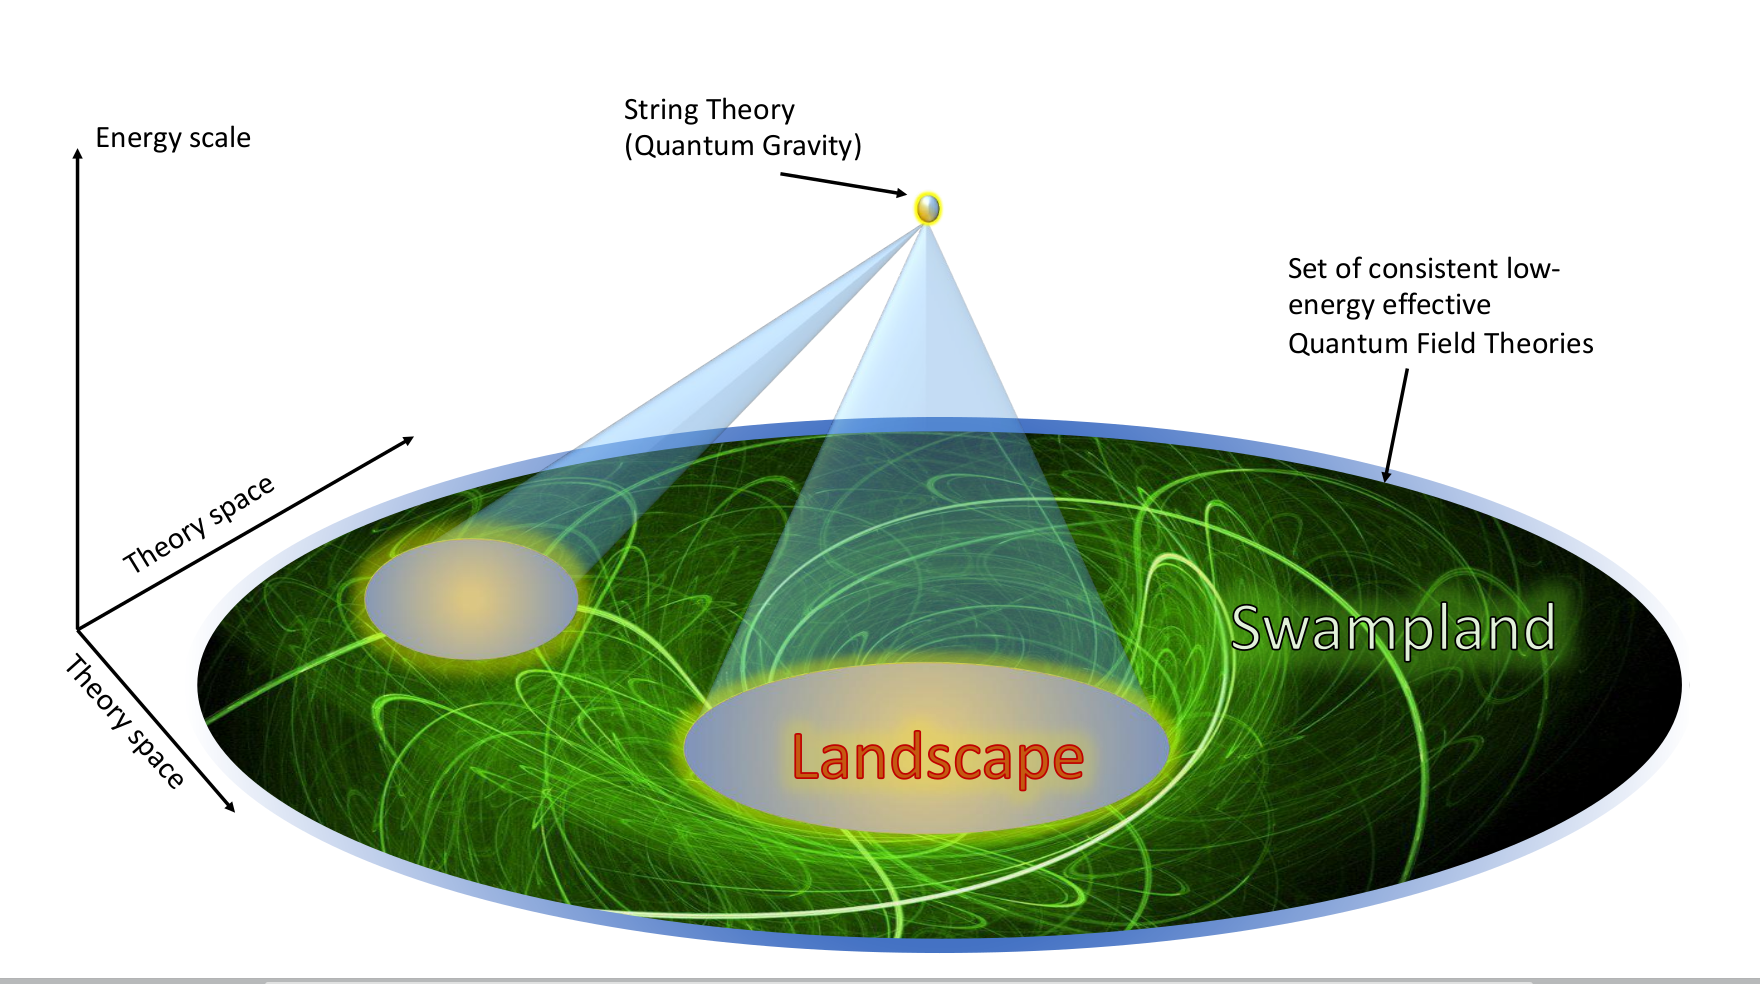
\includegraphics[width=\textwidth]{images/swampland.png}
%     \caption{Landscape and the swampland. Y-axis represents energy scale. Effective field theories in the landscape can be UV completed to string theory. Taken from \citep{Palti:2019pca}}
%     \label{swampland and landscape}
% \end{figure}

In other words, we can complete a low energy theory from the landscape into a UV theory of quantum gravity. But, trying to UV complete a theory form the swampland into a theory of quantum gravity leads to inconsistencies.

\subsection{Swampland distance conjecture}
Whether an effective field theory exists in the swampland or the landscape is the question that swampland conditions try to answer. Although, there are quite a few of these conditions most of them do not have any formal proof from microscopic physics perspective and are thus treated as conjectures. The confidence that we have in these conjectures mostly comes from the observations based on the few known vacua of the string theory and quantum gravity arguments \citep{Brennan:2017rbf}.


% One thing worth mentioning is that the swampland conjectures are defined completely in terms of the low energy effective field theory without any reference to its ultraviolet origin, which implies that the effective field theory has some knowledge about its ultraviolet origin. This is a little unsettling from the renormalization group point of view, which strongly suggests that there is a scale separation in Physics,i.e. low energy theories should not have any knowledge about their ultraviolet counterpart.

One of these conjectures is the swampland distance conjecture (SDC), which states that an effective field theory that has gravity and scalar fields cannot be reliable in the regimes where the scalar field moves beyond an $O(1)$ range.

As we will see in our results, $O(1)$ field movement is observed in the case of black hole formation due to the scalar field collapse. This tension between the SDC and gravitational collapse of a scalar field in general relativity is what we will be exploring in this thesis.
\chapter{Collapse of scalar field in general relativity}


If we have a minimally coupled massless scalar field in general relativity then it will either disperse to infinity or collapse into a black hole. In addition to that if we vary any one parameter $p$ of the initial data then we can find a threshold $p^*$ above crossing which will lead to the formation of a black hole. At this threshold $p^*$ we get critical collapse along with a lot of interesting properties.

Firstly, there is a mass scaling law of the black hole

\begin{equation*}
    M \propto (p - p^*)^\gamma
\end{equation*}

Here M is the mass of the black hole, and $p^*$ depends on the function that describes in the initial data, for example it will be different for a gaussian vs a square initial data. The important point to note here is that $\gamma$ is universal or independent of the the type of the initial data.

This universality has a very important implication, as it implies that one can create a naked singularity because one can effectively create a massless black hole.

Another important property of scalar field collapse close to criticality is called self-similarity. Self-similarity means that close to the origin the scalar field follow a scaling relation,

\begin{equation*}
    \psi(t,x) = \psi(e^{At},e^{Ax})
\end{equation*}

First studies of scalar field collapse were done by Choptuik \citep{Gundlach:2007gc}, but his studies were focussed on the critical collapse.

In our case we were not so much interested in the behavior of the field close to criticality. What we wanted to understand was how much the scalar field moves during the black hole formation so we can relate it to the swampland distance bound.

\section{Scalar collapse equations}


To get the equations of motion we will closely follow the approach taken by \citep{Guo:2018yyt}. We want to study the collapse of minimally coupled scalar field for which the action takes the form,

\begin{equation}
    S=\frac{1}{8 \pi G} \int d^{4} x \sqrt{-g}\left(\frac{1}{2} R-\frac{1}{2} \partial_{\mu} \phi \partial^{\mu} \phi\right)
\end{equation}

Because we want to study the scalar fields near the origin a good choice of coordinates is double-null coordinates,

\begin{equation}
    ds^2=e^{-2 \sigma(t, x)}\left(-d t^{2}+d x^{2}\right)+r^{2}(t, x) d \Omega^{2}
\end{equation}

here $\sigma$ and $r$ are a function of $(t,c)$.

We can now write our equations of motion as,


\begin{equation}
    r\left(-r_{, t t}+r_{, x x}\right)-r_{, t}^{2}+r_{x}^{2}=e^{-2 \sigma}
\end{equation}

\begin{equation}
    -\sigma_{, t t}+\sigma_{,x x}+\frac{r_{, t t}-r_{,x x}}{r}+4 \pi\left(\psi_{, t}^{2}-\psi_{, x}^{2}\right)=0
\end{equation}

\begin{equation}
    -\psi_{, t t}+\psi_{,x x}+\frac{2}{r}\left(-r_{, t} \psi_{, t}+r_{, x} \psi_{, x}\right)=0
\end{equation}

In addition to these evolution equations we also get two constraint equations as well,


\begin{equation}
    r_{, t x}+r_{, t} \sigma_{, x}+r_{, x} \sigma_{, t}+4 \pi r \psi_{, t} \psi_{, x}=0
    \label{eqn:constraint_1}
\end{equation}

\begin{equation}
    r_{, t t}+r_{, x x}+2 r_{, t} \sigma_{, t}+2 r_{, x} \sigma_{, x}+4 \pi r\left(\psi_{, t}^{2}+\psi_{, x}^{2}\right)=0
    \label{eqn:constraint_2}
\end{equation}


Now we introduce a new variable $m$ defined by,

\begin{equation}
    g^{\mu \nu} r_{, \mu} r_{, \nu}=e^{2 \sigma}\left(-r_{, t}^{2}+r_{, x}^{2}\right) \equiv 1-\frac{2 m}{r}
    \label{eqn:m_definition}
\end{equation}

Defining this extra variable helps with the stability of the numerical solutions.
To get the evolution equation for $m$ we differentiate the equation \ref{eqn:m_definition} with respect to time and use the above equations. Using the definition of $m$ we can write the final form of the equations that we will be using to study the scalar collapse,


\begin{equation}
    -\psi_{, t t}+\psi_{, x x}+\frac{2}{r}\left(-r_{, t} \psi_{, t}+r_{, x} \psi_{, x}\right)=0
    \label{eqn:psi}
\end{equation}

\begin{equation}
    -r_{, t t}+r_{, x x}-e^{-2 \sigma} \cdot \frac{2 m}{r^{2}}=0
    \label{eqn:r}
\end{equation}

\begin{equation}
    -\sigma_{, t t}+\sigma_{, x x}-e^{-2 \sigma} \cdot \frac{2 m}{r^{3}}+4 \pi\left(\psi_{, t}^{2}-\psi_{, x}^{2}\right)=0
    \label{eqn:sigma}
\end{equation}

\begin{equation}
    m_{, t}=4 \pi r^{2} \cdot e^{2 \sigma}\left[-\frac{1}{2} r_{, t}\left(\psi_{, t}^{2}+\psi_{, x}^{2}\right)+r_{, x} \psi_{, t} \psi_{, x}\right]
    \label{eqn:m_t}
\end{equation}


differentiating the equation \ref{eqn:m_definition} with respect to $x$ and using the evolution equation we can also get the equation for the $x$ derivative of $m$ which we will be using to solve for the initial conditions.

\begin{equation}
    m_{, x}=4 \pi r^{2} \cdot e^{2 \sigma}\left[\frac{1}{2} r_{, x}\left(\psi_{, t}^{2}+\psi_{, x}^{2}\right)-r_{, t} \psi_{, t} \psi_{, x}\right]
    \label{eqn:m_x}
\end{equation}

\section{Boundary and Initial conditions} \label{chap2:boundary_and_initial_conditions}



There are four variables in our equations $r,m,\sigma,\psi$. At time $t=0$ we only have the value of $\psi$ for all the values of $x$, i.e. we have profile of the initial scalar field configuration. Before we can evolve the system in time we need the profile of other three variable at $t=0$. That being said we are not free to choose any profile for $r,m,\sigma$ because even at $t=0$ they have to satisfy the Einstein equations to represent a physical system.
To get the initial conditions we will use a simplification and set the initial conditions to be time symmetric as follows,

\begin{equation}
    r_{, t}=\sigma_{, t}=\phi_{, t}=\psi_{, t}=0 \quad \text { at } t=0
    \label{eqn:time_symmetric_boundary_conditinons}
\end{equation}

Now we will use equations \ref{eqn:r}, \ref{eqn:constraint_1} and \ref{eqn:m_x} along with the equations \ref{eqn:time_symmetric_boundary_conditinons} to get,


\begin{equation}
    r_{, x x}=e^{-2 \sigma} \cdot \frac{2 m}{r^{2}}
    \label{eqn:r_chap3}
\end{equation}


\begin{equation}
    \sigma_{, x}= -2 \pi \cdot  \frac{\psi_{, x}^{2} \cdot r}{r_{,x}}- e^{-2 \sigma} \cdot \frac{ m}{r^{2}r_{, x}}
    \label{eqn:sigma_chap3}
\end{equation}

\begin{equation}
    m_{, x}=4 \pi r^{2} \cdot e^{2 \sigma}\left[\frac{1}{2} r_{, x} \cdot \psi_{, x}^{2} \right]
\end{equation}

The reason we used equations \ref{eqn:r}, \ref{eqn:constraint_1} and \ref{eqn:m_x} was partially motivated by the fact that we wanted the simplest system that can be solved to get the initial conditions.
We can solve these three ODEs get the initial conditions but we still need the boundary conditions at $(0,0)$ to get that. Here we are just going to mention the boundary conditions that we are going to use, to understand the motivation behind this choice refer \citep{Guo:2013dha}.

\begin{eqnarray}
    r(0 ,0) = 0  \\
    r_{,x}(0 ,0) = 1  \\
    \sigma(0 ,0) = 1  \\
    m(0 ,0) = 1
\end{eqnarray}

Notice that we need four boundary conditions in total and we have them.

To wrap up this chapter we need the boundary conditions at the spatial boundaries. Here we will only derive the boundary conditions at the origin, boundary conditions at the other boundary will be set by extrapolation (more about this choice in the section \ref{chap3:boundary_conditinos}). To get these boundary conditions at the origin we will use regularity arguments.
Observe that $r$ is always set to $0$ at $x=0$, this is done to prevent formation of any kind of cusp at the origin, which give us $r_{,t}(t,0) = 0$ and $r_{,tt}(t,0)=0$.
Now, to ensure that the term $\frac{2}{r}\left(-r_{, t} \psi_{, t}+r_{, x} \psi_{, x}\right)$ from the equation \ref{eqn:psi} is regular at the origin we need that $r_{, x} \psi_{, x}$, because $r_{,t}(t,0)$ is already $0$, which give us that $\psi_{,x}(t,0) = 0$. Looking at the equation \ref{eqn:m_definition} we can also see that we need $m(t,0) = 0 $. Similarly from the equation \ref{eqn:r} we get that $r_{,xx}=0$. Finally, at the origin the equation \ref{eqn:constraint_2} becomes $r_{,x} \sigma_{,x} = 0$ which gives us $\sigma_{,x}(t,0) = 0$.


During the numerical evolution we will need the following boundary conditions,

\begin{eqnarray}
    r(t,0) = 0 \\
    m(t,0) =0 \\
    \psi_{,x}(t,0) = 0\\
    \sigma_{,x}(t,0) = 0
\end{eqnarray}

\chapter{Solving Einstein Equations}

While studying gravitational collapse of a scalar field we got a set of differential equations. These differential equations were complicated enough that any effort to find an analytical solution was futile. One can always make some approximations and get some understanding of the solutions, but to get a complete solution we need to use numerical techniques. In this chapter we will discuss about how to solve differential equations on a computer.




\section{Finite difference methods}

Solving differential equations is required in almost every field of Science and although analytical solution are the best thing one can get, they are hard to come by.
Most of the time we have to resort to solving differential equation numerically. There a lot of methods out there developed to solve differential equations, each of them have their own advantages and dis-advantages. In our case we will be using a class of methods called finite difference methods.

\index{Finite difference methods} Finite difference methods are the most intuitive and easy to implement methods. They are derived using the taylor series and give a discrete approximation of the strong from of the differential equations.

To get some intuition about finite difference methods let us start with a very simple example. These simple examples will demonstrate some of the most important concepts of finite difference computing.

Suppose that we want to find the value of the derivative of the function $f(x) = x^3$ at $x =1$. We know that the answer should be $3$. But, let us say that we do not know the exact formula and want to approximate the derivative.
The simplest way to do this would be using the formula of the derivative itself,

\begin{equation}
    \frac{dy(x_0)}{dx} = \lim_{h \to 0}\frac{y(x_0 + h) - y(x_0)}{h}
\end{equation}

The definition of derivative gives us the exact answer in the limit. What we can do is to take $h$ to a small non-zero number and see if that gives us an approximate answer.

\begin{equation}
    \frac{dy(x_0)}{dx} \approx \frac{y(x_0 + h) - y(x_0)}{h} , \text{for } h << 1
\end{equation}\label{eq:first_order}

We have shown the results of using the equation \ref{eq:first_order} to approximate the derivative of $x^3$ at $x=1$ in the figure \ref{fig:x^3_error_order1}. Y axis in the figure is the log error of the approximation and X axis is the log of the \index{step size} step size ($h$). Figure \ref{fig:x^3_error_order1} has a lot of stuff going on in it and we will break it down into parts. But before we do that we will briefly look at how computers store decimal numbers and how does it affect our calculations.

\subsection{Floating point arithmetic}

\index{Floats} Floats are how computers internally represent decimal numbers. A larger sized float can handel both a larger number and more significant digits\index{significant digits}. Because computers can only stores a fixed number of digits after the decimal point we get \index{floating point errors} floating point errors whenever any calculation is done on these floats. For example we know that $\frac{1}{3}$ has a recurring decimal expansion, but if we want to save $\frac{1}{3}$ in the computer, in its decimal representation, then there will be a small error because we can only store a fixed number of significant digits.




\begin{table}[hbt!]
    \centering
    \begin{tabular}{||m{2cm} | m{3.2cm} | m{1.5cm} | m{4.5cm}||}
        \hline
        Float type & Largest Number that can be stored* & Precision & How is $\frac{1}{3}$ internally stored \\ [0.5ex]
        \hline\hline

        Float32    & 3.40e+38                           & 6         & 0.33333334                             \\

        Float64    & 1.79e+308                          & 15        & 0.3333333333333333                     \\

        Float128   & 3.36e+4932                         & 18        & 0.33333333333333333334                 \\ [1ex]
        \hline
    \end{tabular}
    \caption{This table shows the largest number that can be represented by a particular type of float (* rounded off to two decimal places). Precision denotes the number of significant decimal digits that can be represented by a float type.}
    \label{table:floats}
\end{table}

Table \ref{table:floats} has the information about different kind of floats used in the graphs. \index{Precision}Precision denotes the number of significant digits that a particular type of float can store, for example, float32 can store just 6 numbers after the decimal point which is why $\frac{1}{3}$ is stored as $0.33333334$. Also, note that the there is a huge difference in the largest number that can be stored between different kind of floats. If we try to store a number larger than the maximum number that a float type can hold we get an overflow error and computer starts giving us random garbage. Different languages and libraries deal with such errors in different ways and it is not worth going into the specifics, but the bottom line is that we can not work with float64 if our systems have numbers larger than $1.79*10^{308}$.


Most of the modern computers chips use float64 internally and they have CPU circuits that are very efficient in working with float64 numbers. Float64 denotes that this number will use 64bits of memory, while float32 numbers only use 32bits of memory; this means that we can store more float64 numbers in the same amount of memory. What this means in practical terms is that a we can store around $10^9$ floats in $8GB$ of RAM, or a matrix with approximately 31000 rows and columns. If we are not clever with what we are storing in our RAM there is real danger that we may run out of memory, which will cause an error and our program will stop.


Among the parameters listed in Table \ref{table:floats} the most important parameter for any calculation is the precision. As already mentioned whenever we perform any kind of operation on a floating point number there is an error due to the \index{finite precision}finite precision of floating point numbers.
We can see this phenomenon quite easily just by adding $1.0$ to $\frac{1}{3}$ stored as a float32. If we add $1.0$ to $0.\overline{33}$, $10000$ times the expected answer is $10000.\overline{33}$ which in float32 precision should be $10000.3333334$. But, we see that the actual answer that we get is $10000.334$, that is we have lost 4 significant digits.
This loss of accuracy is what we call \index{floating point error}floating point error and this is the reason why using float32 for numerical computations is a bad idea. If we use float64 instead of float32 we will still lose 4 significant digits but it will not so much because we will still have 11 significant digits in the decimal to work with. We should mention here that there is no hard and fast formula for how many digits will we lose per operation and it depends on the language and libraries used as many of them are optimized to reduce floating point errors.\label{para:addition_errors}

We will discuss one final point we need to discuss before we wrap up this section and go back to developing finite difference algorithms. Given any two floating point numbers, we want to ask that when are they equal to each other?
This question is important because it is related to the precision of floating point numbers. For example, if we try to subtract $1.0000001$ from $1.0000007$ and they are stored as float32, then we will get some random garbage. The reason being that float32 can not handle more than 6 decimal significant digits properly.
The general rule is that one should try to avoid subtracting two numbers that are close and have a lot of significant digits in their \index{mantissa}mantissa, as that usually gives a lot of error.
Just for the sake of clarity, we should mention that here we are not taking about numbers with small magnitude. So, even float32 can easily handle numbers of small magnitude like subtracting $2*10^{-30}$ from $1*10^{-30}$ because their mantissa does not have a lot of significant digits. But, at the same time $2 + 10^{-8}$ and $2$ will both be stores as $2.0$ inside the computer memory and will give zero if subtracted from each other.


Here we have given all the examples in float32 but the concepts carry over to float64, the only difference being that float64 can handle much smaller number and more significant digits. As already mentioned modern computers CPU's are designed to deal with float64 arithmetic and it is accurate enough so we use it for most of our calculations. Using float128 or larger floats can give much more accuracy but they will very slow compared to using float64 and are not required for most of the applications.

\subsection{Floating point errors in finite difference approximations}

Now that we have some idea about the floating point arithmetic we can dive into the graphs.
In the figure \ref{fig:x^3_error_order1} there are three lines, each corresponding to a different sized float used for the calculations.

To approximate the derivative of $x^3$ at $x=1$ we have used the formula,

\begin{equation}
    \frac{dy(x_0)}{dx} \approx \frac{y(x_0 + h) - y(x_0)}{h} , \text{for } h << 1
\end{equation}\label{eq:first_order_2}

This is called a \index{first order} first order finite difference approximation. To understand why is it called we will taylor expand the $y(x)$ around $x_0$ with step size $h$

\begin{equation}
    y(x_0 + h) = y(x_0) + y'(x_0)*h +\frac{y''(x_0)*h^2}{2} + \dots
\end{equation}

If we truncate the series at $O(h^2)$ and rearrange a little we get,

\begin{equation}
    y(x_0 + h) - y(x_0) \approx y'(x_0)*h +\frac{y''(x_0)*h^2}{2}
\end{equation}

dividing by $h$ we get,

\begin{equation}
    y'(x_0)  \approx \frac{y(x_0 + h) - y(x_0)}{h} - \frac{y''(x_0)*h}{2}
\end{equation}

Notice that this is the exact formula that we were using for approximating the derivative except for the presence of the extra term $\frac{y''(x_0)*h}{2}$. This extra term represents the error in our approximation (there are of course other higher order terms that we ignored, but this term is going to dominate them anyways). Because the error falls off with the step size $h$ we call this a first order approximation. Looking at the figure \ref{fig:x^3_error_order1} this becomes clear, if the step size was decreased by a factor of two then the error will also go down by a factor of two, i.e. slope of the log(error) vs log(h) line will have a slope 1.

\begin{figure}[hbt!]
    \centering
    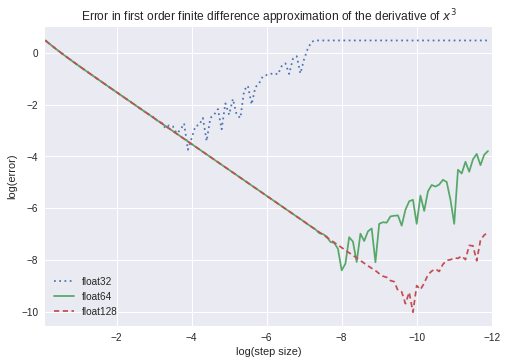
\includegraphics[width=\textwidth]{images/x^3_error_order1.png}
    \caption{This plot show error of using finite difference to approximate the derivative of $x^3$ vs the step size. Observe that the error falls almost linearly until the floating point errors start to dominate, after which it starts to grow erratically. Also, observe that for reasonable step sizes the error falls with a slope of 1, which is why such approximations are called to be of first order. }\label{fig:x^3_error_order1}
    \index{figures}
\end{figure}

In the beginning, irrespective of the float size, we have a straight line which turns into a wiggly mess as we keep on decreasing the step size. The reason for this sudden increase in the error is floating point errors. One can clearly see that going form float32 to float64 is a big jump in accuracy. But going to float128 from float64 the increase in the accuracy is not so dramatic, which is kind of expected as float128 has only 3 more significant digits over float64.

We can also use higher order methods, for example a second order method,

\begin{equation}
    y'(x_0)  \approx \frac{y(x_0 + h) - y(x_0 - h)}{2*h}
\end{equation}\label{eq:d_second_order}

To show that this a second order method one can taylor expand $y(x)$ around $x_0$ with step size $h$ and $-h$ and plug it back into the equation \ref{eq:d_second_order}. Figure \ref{fig:x^3_error_order2} shows the log(error) vs log(step size) graph for the second order approximation, notice that the slope of the line is now 2. Using higher order methods can give more accurate results for the same step size but they lead to other issues which we will briefly discuss later.

\begin{figure}[hbt!]
    \centering
    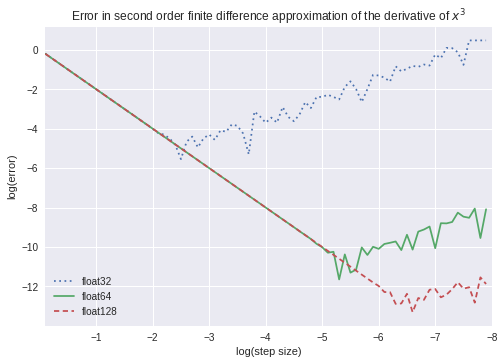
\includegraphics[width=\textwidth]{images/x^3_error_order2.png}
    \caption{This plot show error of using finite difference to approximate the derivative of $x^3$ vs the step size. Observe that the error falls almost linearly until the floating point errors start to dominate, after which it starts to grow erratically. Also, observe that for reasonable step sizes the error falls along a line with slope 2 which is to be expected of a second order approximation. }\label{fig:x^3_error_order2}
    \index{figures}
\end{figure}


To give some perspective, while solving the scalar collapse equations we are going to use step size of the order $10^{-5}$, thus using float32 is just out of the picture. Which implies that there will be at least $10^{5}$ operations per element (we can not decrease spatial step size without decreasing the time step size at the same time, something we will explore more in the next sections). From the discussion in the section \ref{para:addition_errors} we know that there is an error associated with each operation as well, thus even though individual errors may be small but given the size of calculations we are interested in they can quickly add up and destroy our simulations.







\begin{figure}[hbt!]
    \centering
    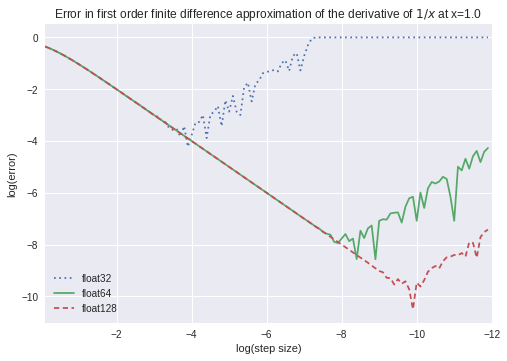
\includegraphics[width=0.8\textwidth]{images/1_x_error_at_1.png}
    \caption{This plot show error of using finite difference to approximate the derivative of $\frac{1}{x}$ vs the step size.}\label{fig:1/x_1}
    \index{figures}
\end{figure}

\begin{figure}[hbt!]
    \centering
    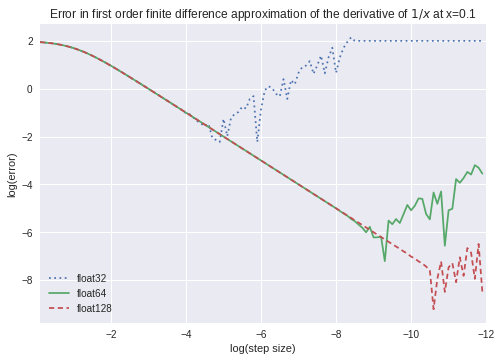
\includegraphics[width=0.8\textwidth]{images/1_x_error_at_p1.png}
    \caption{This plot show error of using finite difference to approximate the derivative of $\frac{1}{x}$ vs the step size.}\label{fig:1/x_0.1}
    \index{figures}
\end{figure}


\begin{figure}[hbt!]
    \centering
    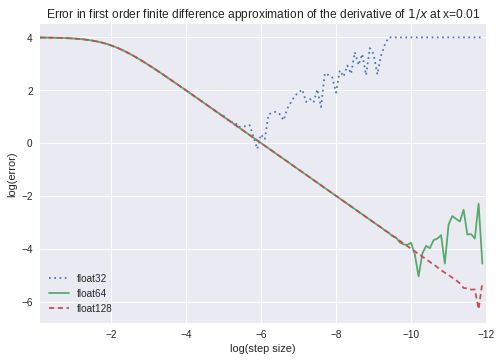
\includegraphics[width=0.8\textwidth]{images/1_x_error_at_p01.png}
    \caption{This plot show error of using finite difference to approximate the derivative of $\frac{1}{x}$ vs the step size.}\label{fig:1/x_0.01}
    \index{figures}
\end{figure}
\chapter{Profiles used and results}
Most of this chapter is taken from \citep{Chaudhary:2020yyv}.

For all these profiles we the spatial domain was [0,2] and the time domain was [0,1].
We used four different profiles of $\psi$,


Gaussian profile:
\[
    \psi(t=0, x)=A \exp \left(\frac{-\left(x-x_{0}\right)^{2}}{\delta^{2}}\right)
\]

Maxwell (or Modified Gaussian) profile:
\[
    \psi(t=0, x)=A x^{2} \exp \left(\frac{-\left(x-x_{0}\right)^{2}}{\delta^{2}}\right)
\]

Ball (or tanh) profile:
\[
    \psi(t=0, x)=A\left(\tanh \left(\frac{-\left(x-x_{0}\right)}{\delta^{2}}\right)+1\right)
\]

Shell profile:
\[
    \psi(t=0, x)=A\left(\tanh \left(\frac{-\left(x-x_{0}\right)}{\delta^{2}}\right)+\tanh \left(\frac{\left(x-x_{0}+w\right)}{\delta^{2}}\right)\right)
\]

For all these profiles we first obtained a rough estimate of the critical amplitude, which was then used to evolve the system once with a subcritical amplitude and then again with a supercritical amplitude.

The simulation was evolved in the supercritical case when it was obvious that the scalar field has moved by $O(1)$ in plank units.

For each profile we are showing two figures, figure (a) shows the fields evolution in time. Blue line is the initial value of $\psi$, green is the value of the field when it reached its maxima at the origin and red is the final value of the field before we stopped the simulation (We stopped the simulations when it was apparent that the field has moved by $O(1)$ distance). Figure (b) shows the value of the field at the origin vs time, blue line shows the subcritical evolution and red line shows the supercritical evolution.

To gain confidence in the results we ran the simulations with multiple step sizes to ensure that the results are independent of the algorithm. In addition to that we also checked the two constraint equations to ensure that the system us evolving correctly.

Subcritical evolution does not involve a lot of field movement thus our algorithm gives very accurate results. But, in the supercritical cases during the collapse the fields start to move very rapidly which leads to a lot of error \ref{chap3:floating_point_errors}.
For the gaussian and the modified gaussian case the constraints had values of the order $10^-5$ at the end.
For the square and the shell profiles the value of the constraint were of the order $10^-3$ at the end of the simulation. These comparatively larger values can be attributed ot the fact that during the collapse field moves much faster in case of square and the shell profiles (Figures \ref{fig:at0_modified_gaussian},\ref{fig:at0_modified_gaussian},\ref{fig:at0_tanh},\ref{fig:at0_shell}).
Although, even in supercritical cases when the field was not moving very fast the constraints were much smaller.

We can decrease the step size to get more accurate results but there is limit on how small one can go due to fixed finite RAM size. One way to deal with this is to use adaptive mesh refinement(AMR), where one reduces the step size at the places where the field is moving very fast to get more accurate results. We decided not to use AMR because writing a AMR code is significantly harder and the accuracy that we were able to achieve was enough to demonstrate our point. That being said with more powerful computers and better algorithms it is possible to achieve much better accuracies if required.



\begin{figure}
    \centering
    \begin{subfigure}[b]{0.85\textwidth}
        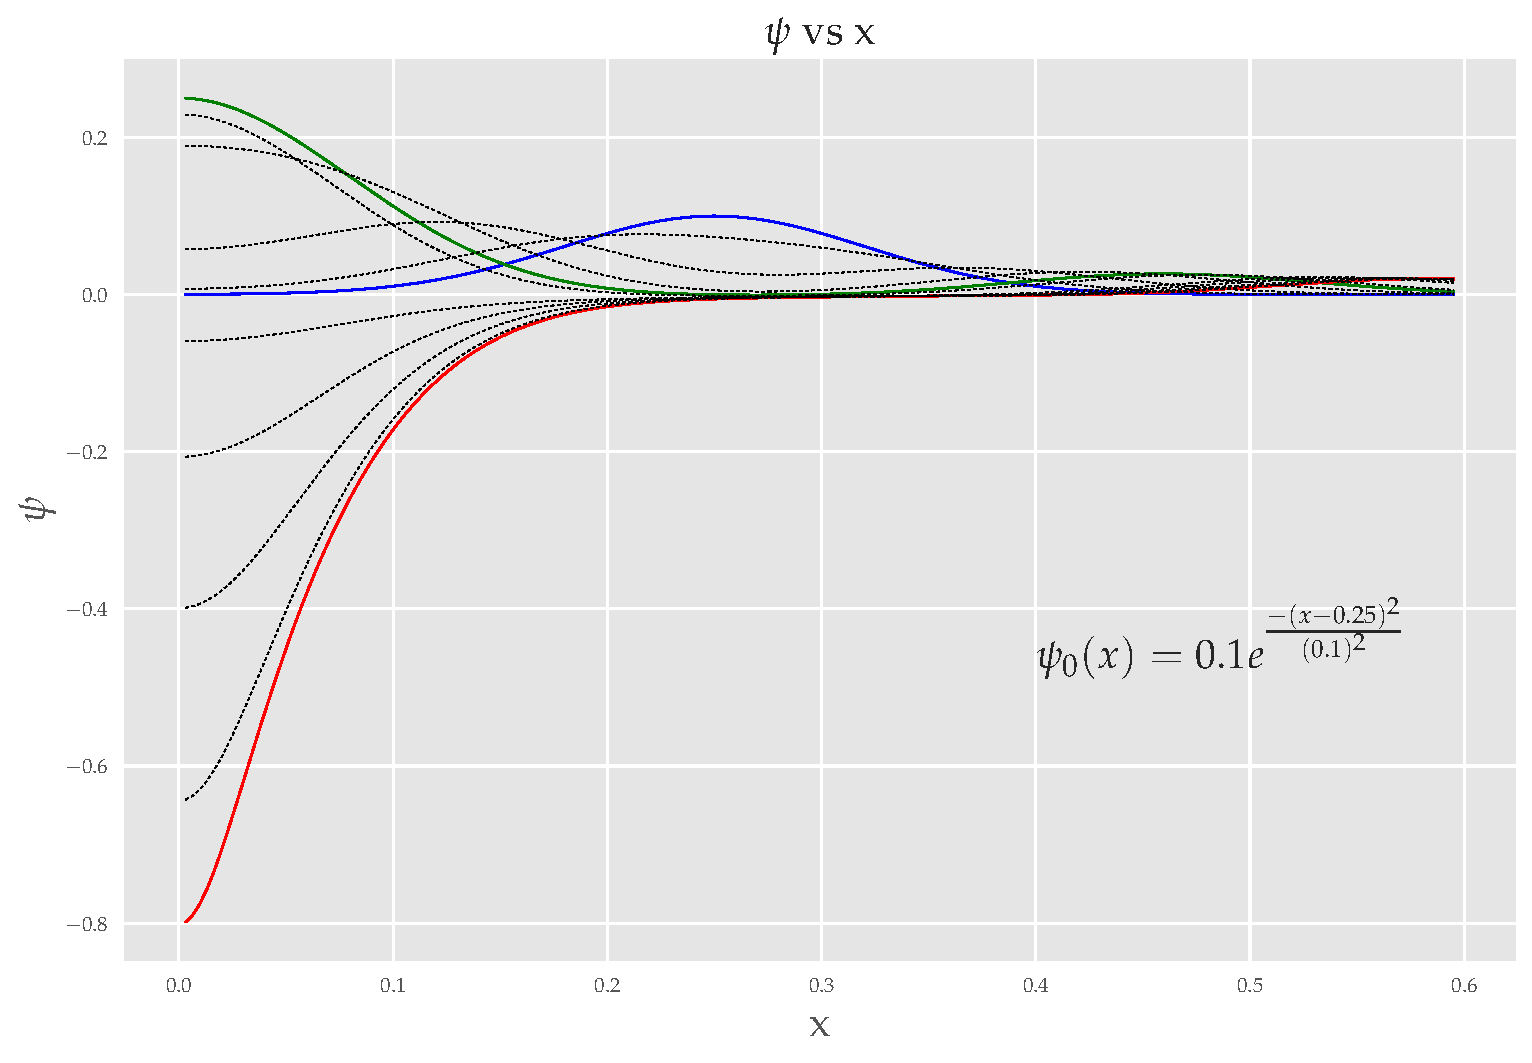
\includegraphics[width=1\linewidth]{images/super_Gaussian.pdf}
        \caption{}
        \label{fig:Ng1}
    \end{subfigure}

    \begin{subfigure}[b]{0.85\textwidth}
        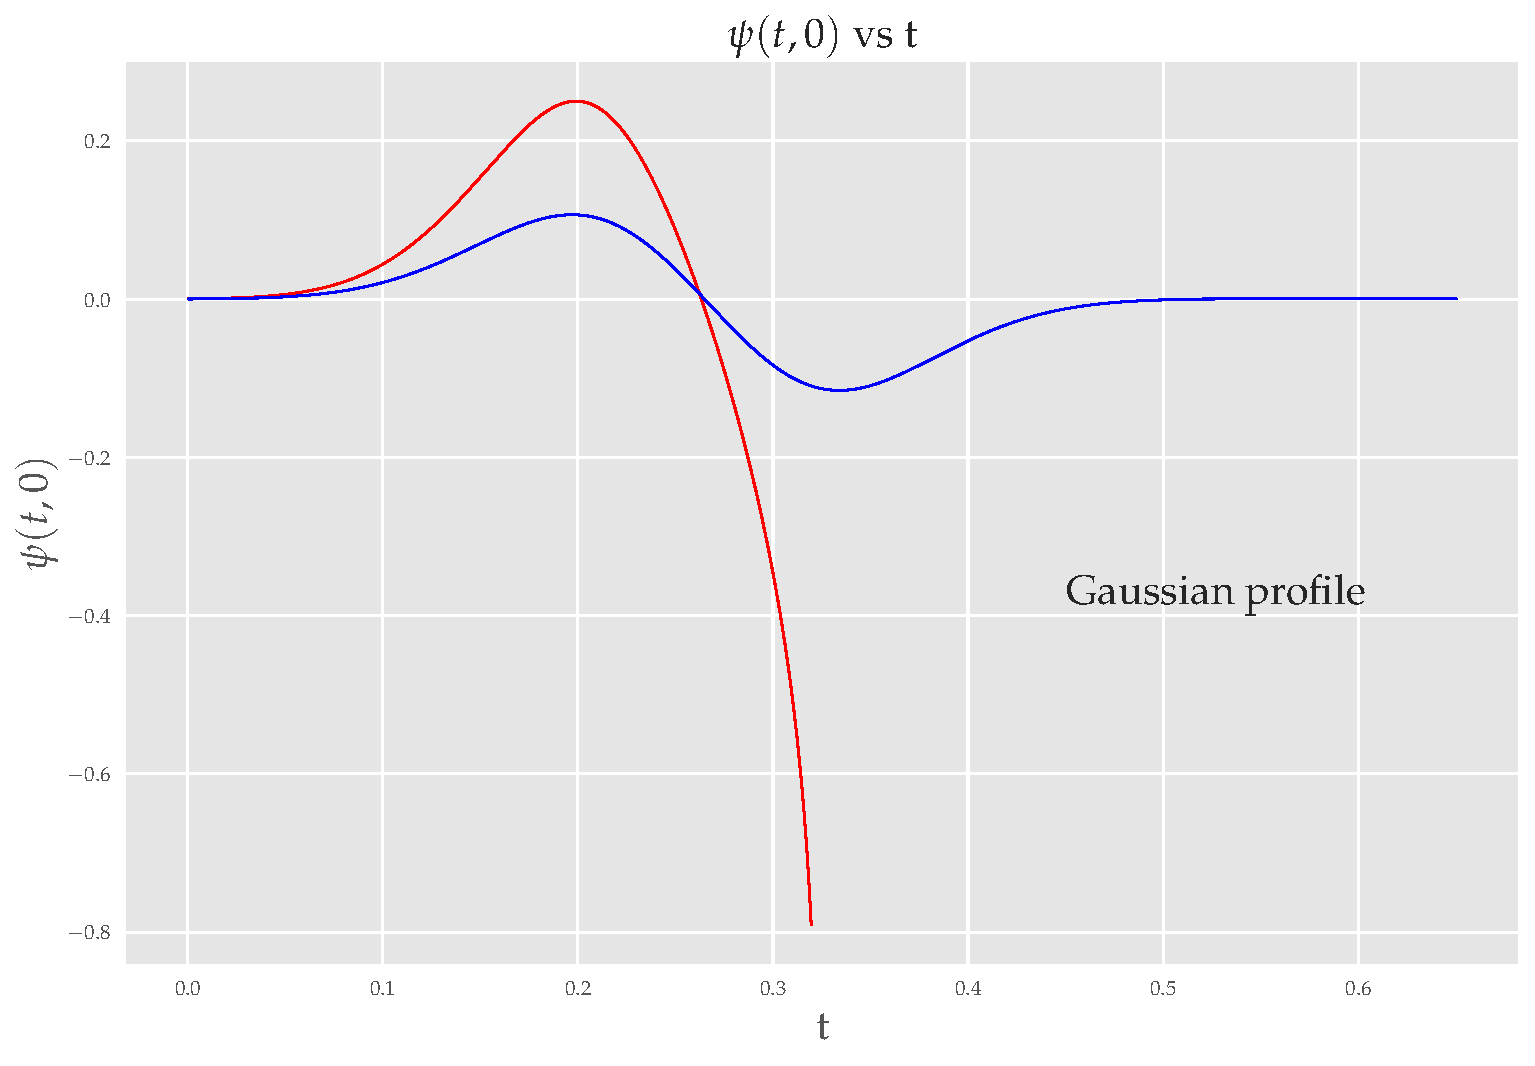
\includegraphics[width=1\linewidth]{images/at0_Gaussian.pdf}w
        \caption{}
        \label{fig:Ng2}
    \end{subfigure}
    \caption[Gaussian profile field evolution]{\textbf{Gaussian Profile}. Figure (a) shows supercritical evolution of the field, \textbf{Blue}: initial profile of $\psi$ , \textbf{Green}: profile of $\psi$ when $\psi$ reaches its maxima at the origin, \textbf{Red}: final profile of $\psi$ before the simulation was stopped. Figure (b) shows the supercritical (\textbf{red}) and the subcritical (\textbf{blue}) evolution of $\psi$ at the origin with respect to time.}
\end{figure}



\begin{figure}
    \centering
    \begin{subfigure}[b]{0.85\textwidth}
        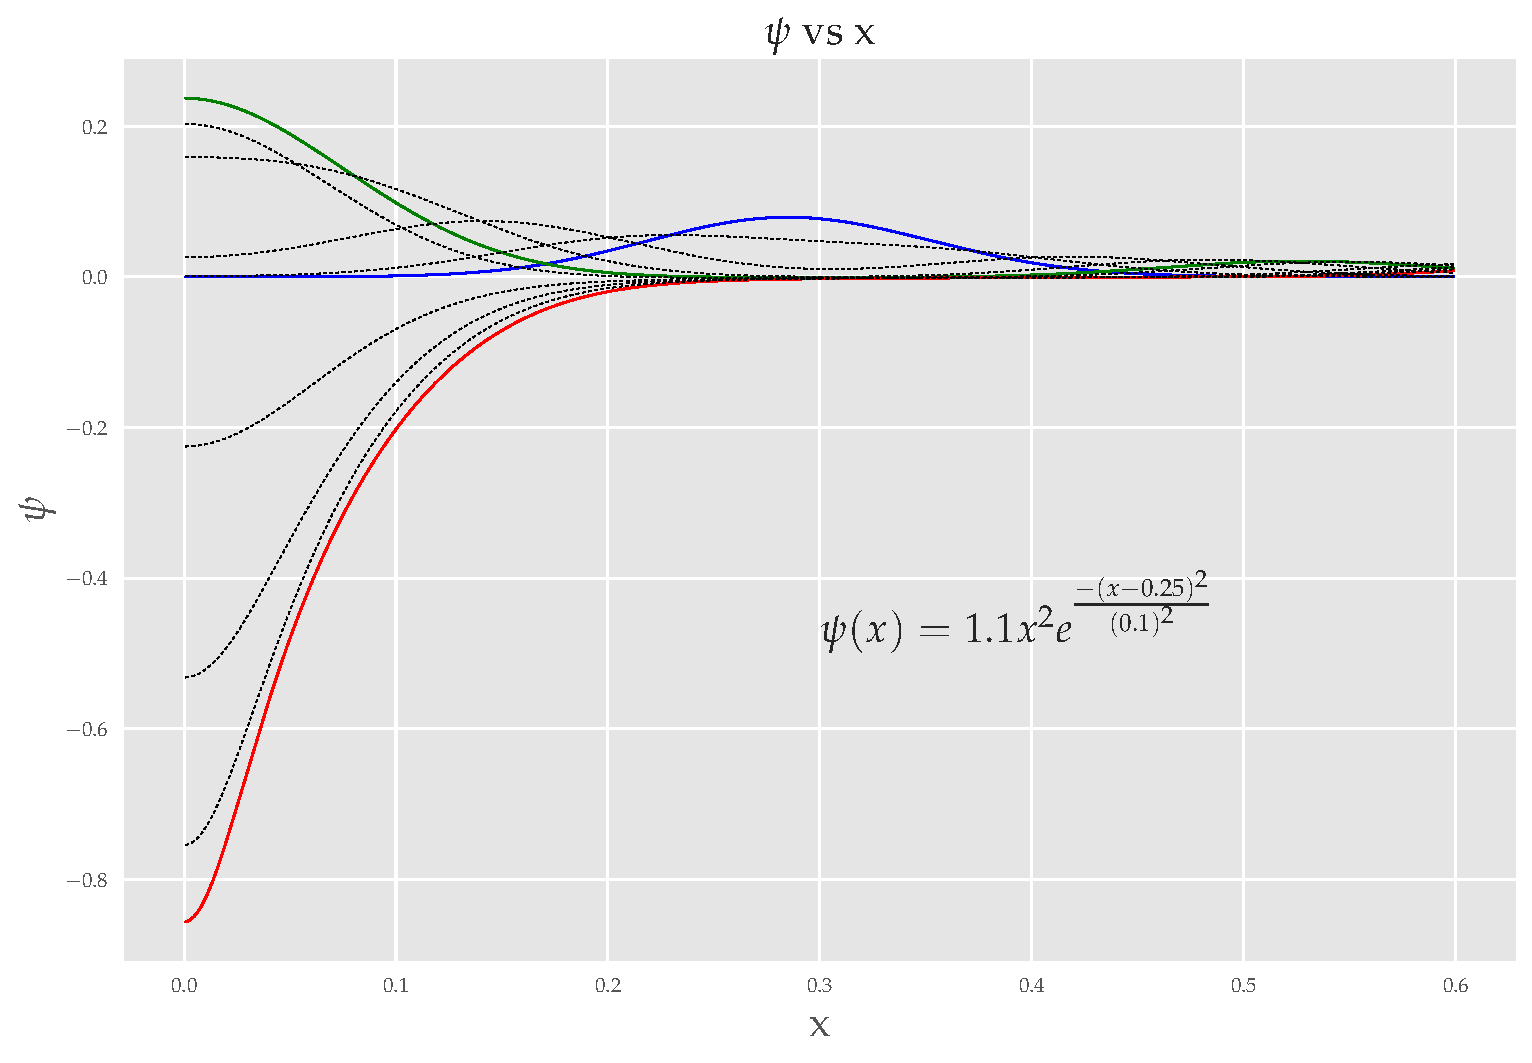
\includegraphics[width=1\linewidth]{images/super_mod.pdf}
        \caption{}
        \label{fig:modified_gaussian}
    \end{subfigure}

    \begin{subfigure}[b]{0.85\textwidth}
        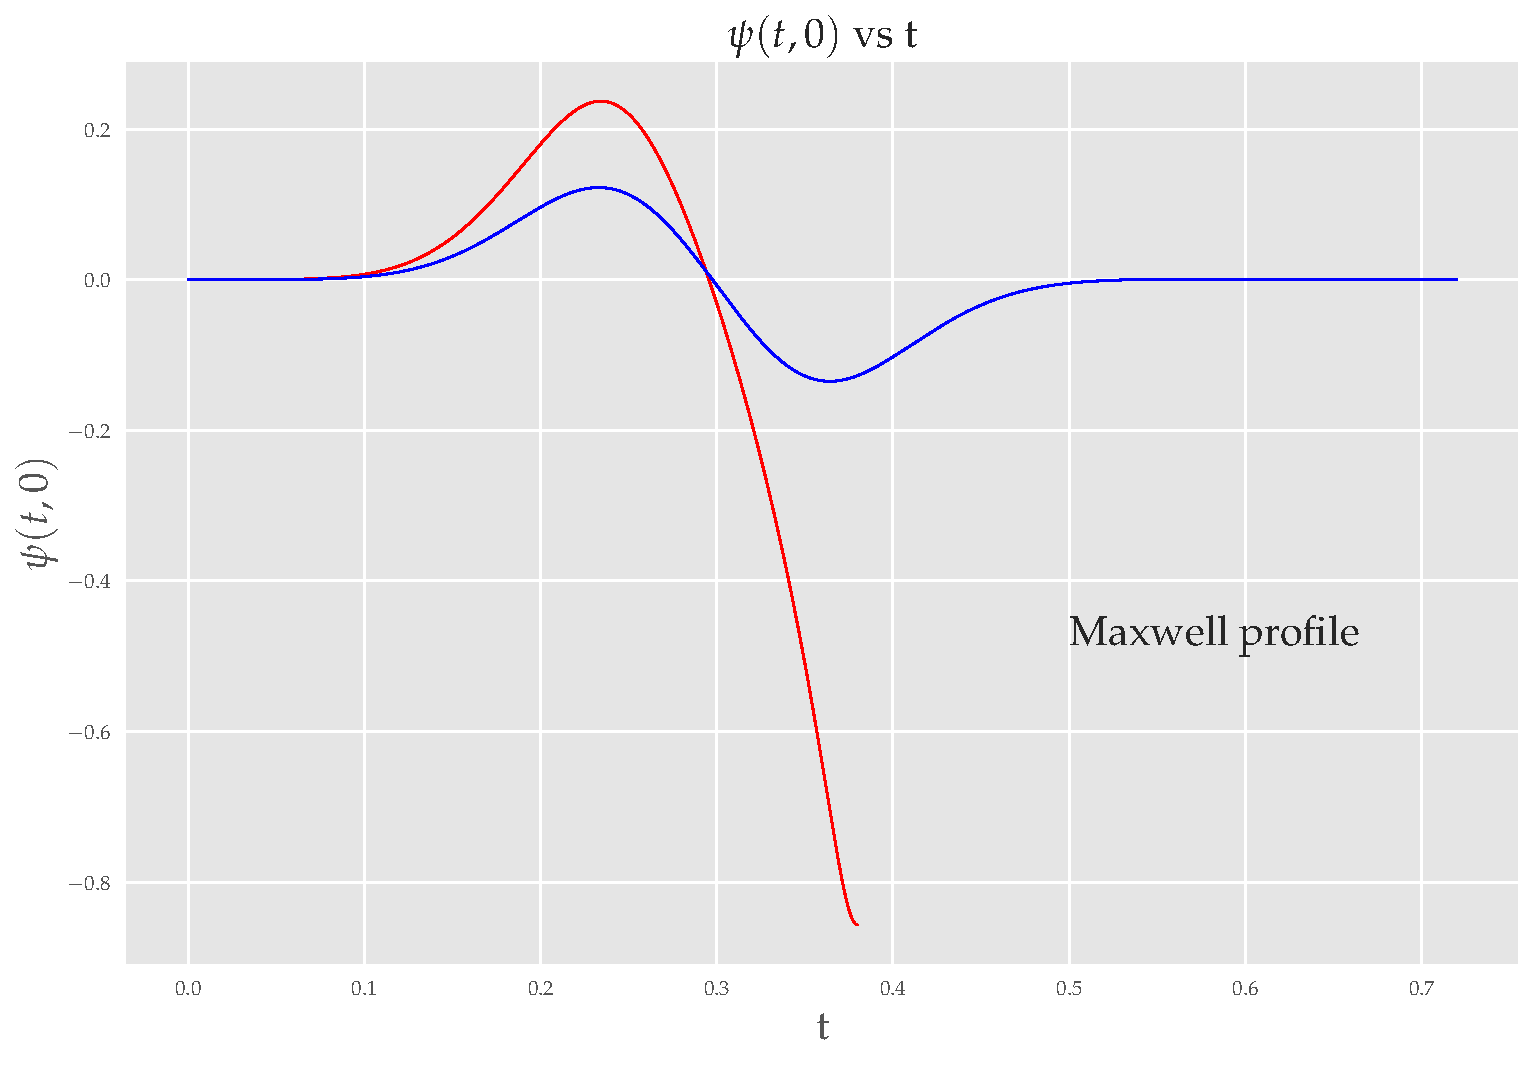
\includegraphics[width=1\linewidth]{images/at0_mod.pdf}
        \caption{}
        \label{fig:at0_modified_gaussian}
    \end{subfigure}
    \caption[Modified Gaussian profile field evolution]{\textbf{Maxwell Profile}. Figure (a) shows supercritical evolution of the field, \textbf{Blue}: initial profile of $\psi$ , \textbf{Green}: profile of $\psi$ when $\psi$ reaches its maxima at the origin, \textbf{Red}: final profile of $\psi$ before the simulation was stopped. Figure (b) shows the supercritical (\textbf{red}) and the subcritical (\textbf{blue}) evolution of $\psi$ at the origin with respect to time.}
\end{figure}

\begin{figure}
    \centering
    \begin{subfigure}[b]{0.85\textwidth}
        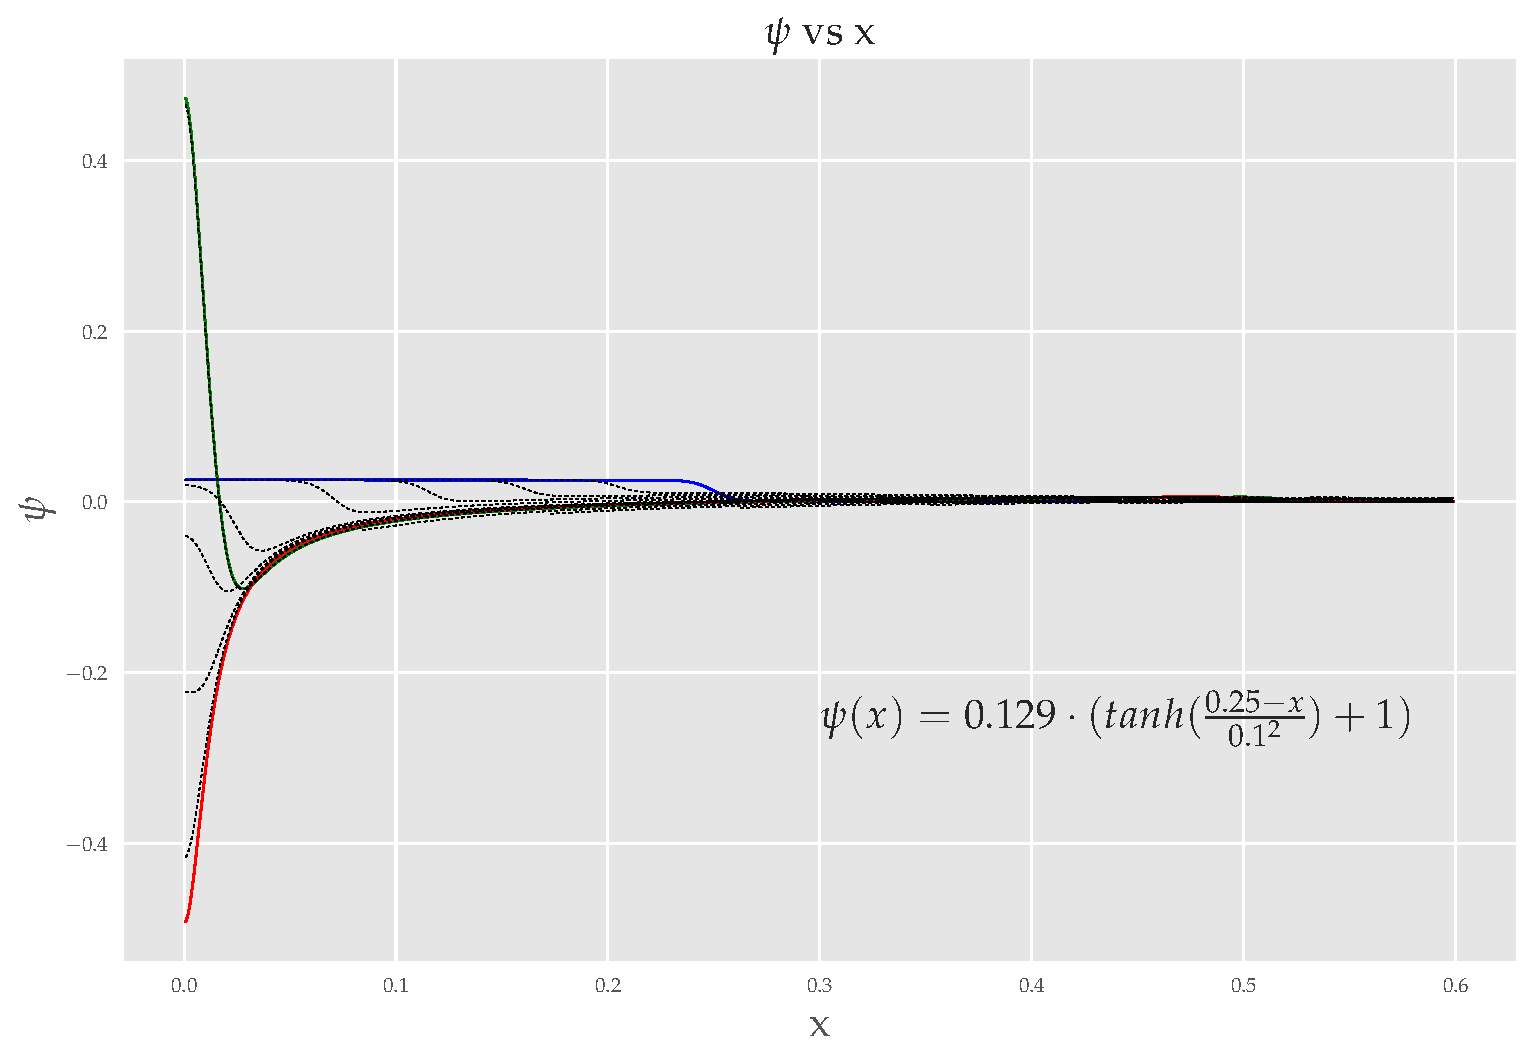
\includegraphics[width=1\linewidth]{images/super_tanh.pdf}
        \caption{}
        \label{fig:tanh}
    \end{subfigure}

    \begin{subfigure}[b]{0.85\textwidth}
        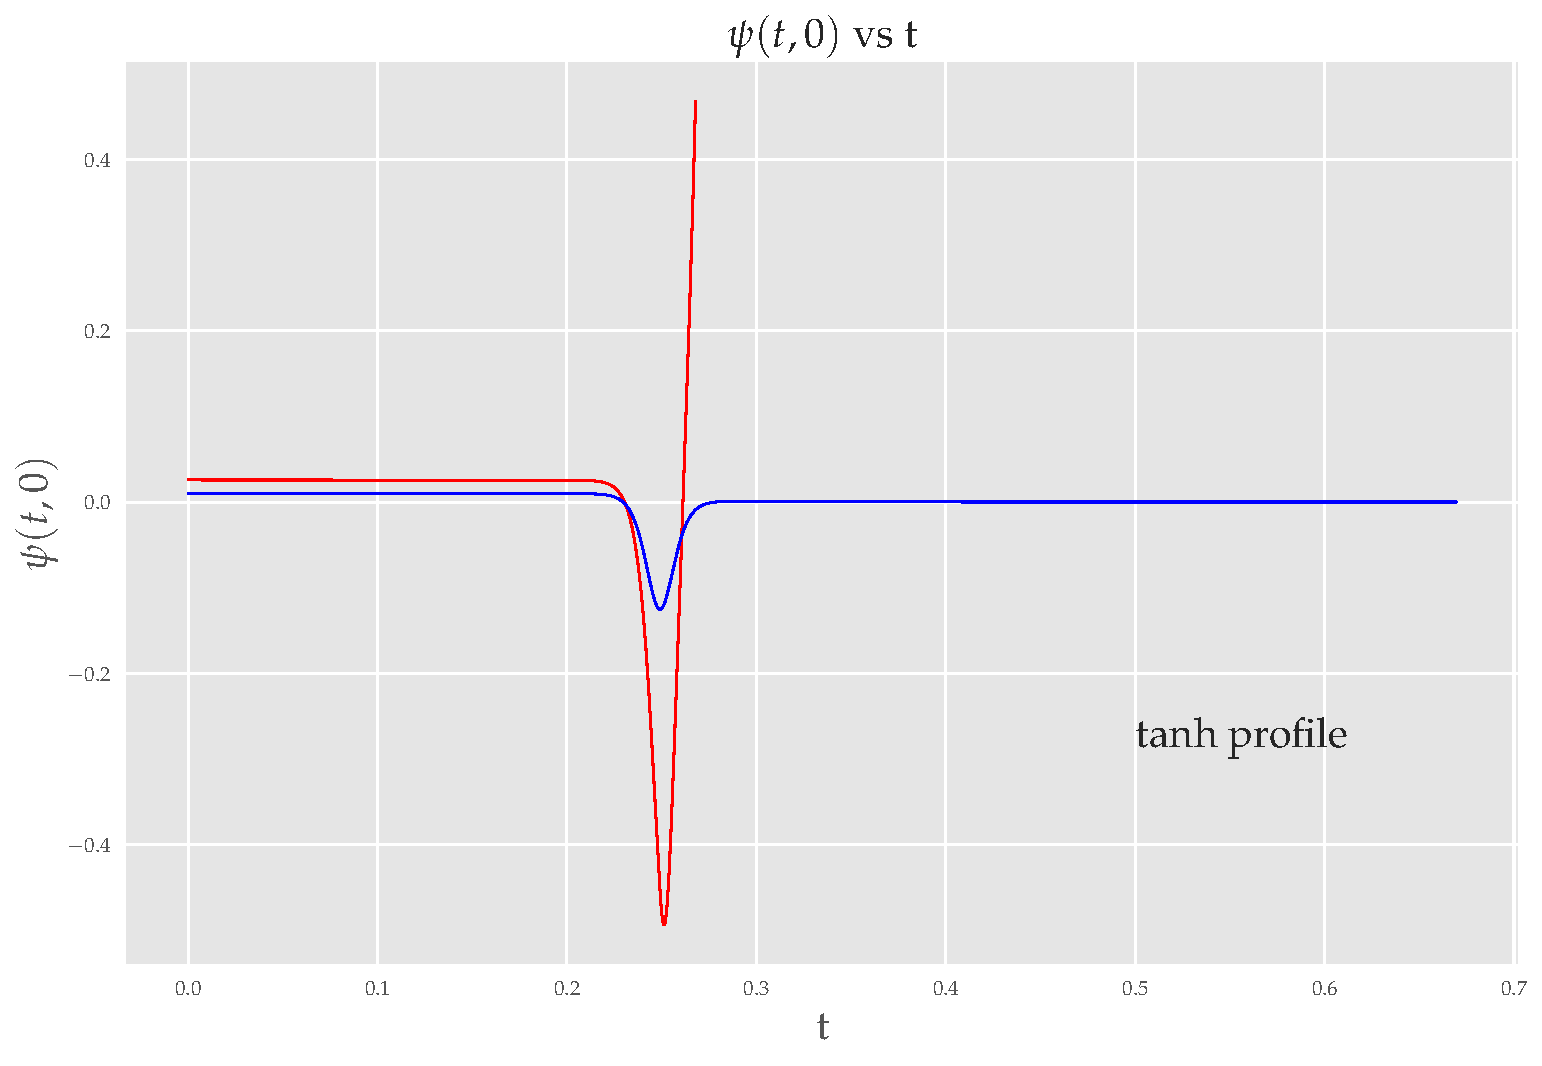
\includegraphics[width=1\linewidth]{images/at0_tanh.pdf}
        \caption{}
        \label{fig:at0_tanh}
    \end{subfigure}
    \caption[tanh profile field evolution]{\textbf{Tanh Profile}. Figure (a) shows supercritical evolution of the field, \textbf{Blue}: initial profile of $\psi$ , \textbf{Green}: profile of $\psi$ when $\psi$ reaches its maxima at the origin, \textbf{Red}: final profile of $\psi$ before the simulation was stopped. Figure (b) shows the supercritical (\textbf{red}) and the subcritical (\textbf{blue}) evolution of $\psi$ at the origin with respect to time.}
\end{figure}

\begin{figure}
    \centering
    \begin{subfigure}[b]{0.85\textwidth}
        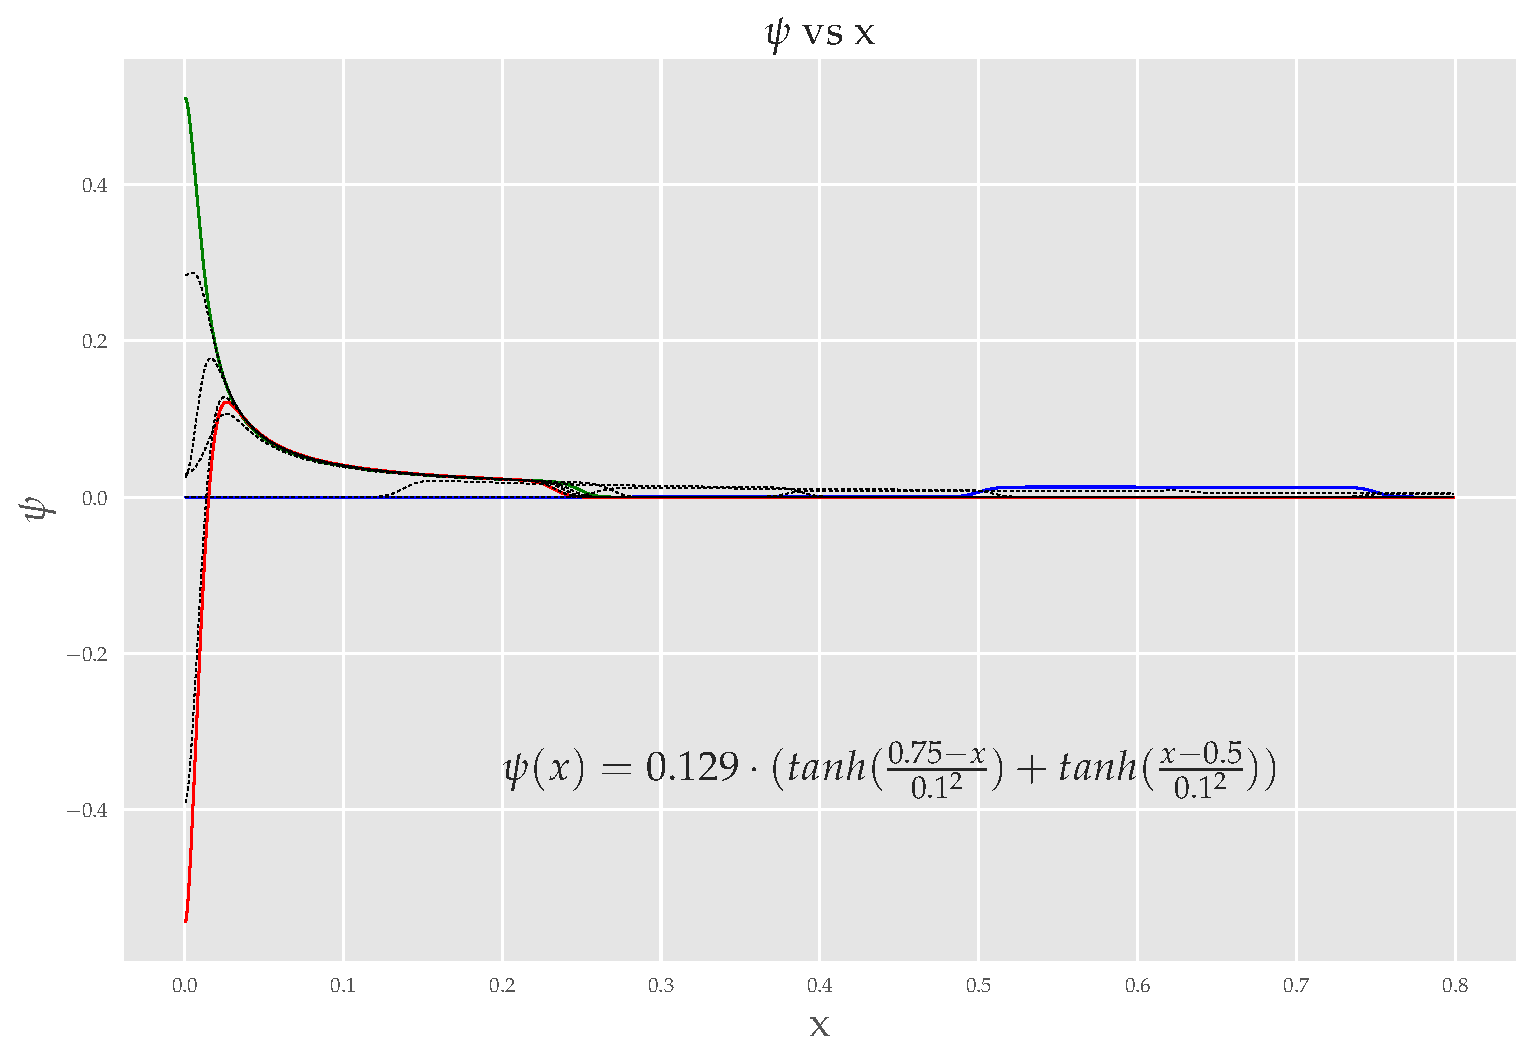
\includegraphics[width=1\linewidth]{images/super_shell.pdf}
        \caption{}
        \label{fig:shell}
    \end{subfigure}

    \begin{subfigure}[b]{0.85\textwidth}
        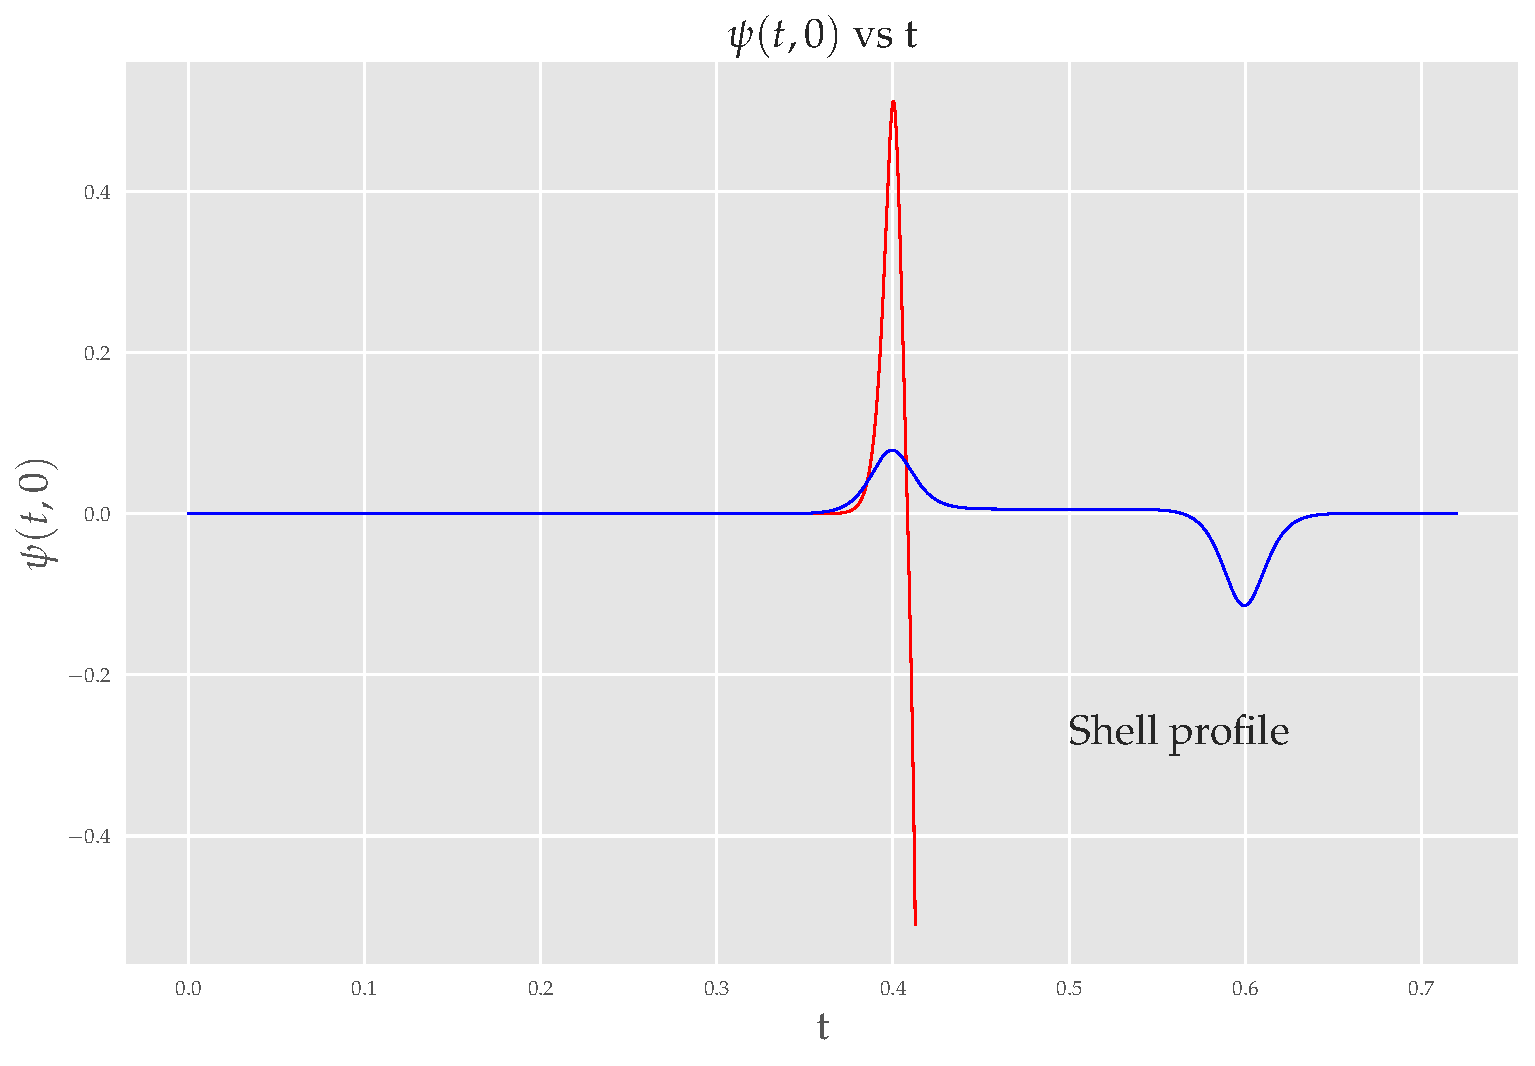
\includegraphics[width=1\linewidth]{images/at0_shell.pdf}
        \caption{}
        \label{fig:at0_shell}
    \end{subfigure}
    \caption[shell profile field evolution]{\textbf{Shell Profile}. Figure (a) shows supercritical evolution of the field, \textbf{Blue}: initial profile of $\psi$ , \textbf{Green}: profile of $\psi$ when $\psi$ reaches its maxima at the origin, \textbf{Red}: final profile of $\psi$ before the simulation was stopped. Figure (b) shows the supercritical (\textbf{red}) and the subcritical (\textbf{blue}) evolution of $\psi$ at the origin with respect to time.}
\end{figure}

\chapter{Results}
% \chapter{Conclusions and Future Directions}

\printbibliography[heading=bibintoc]

\appendix

% \chapter{Derivations}
% \chapter{Other methods of solving differential equations}
% \chapter{Pade` methods}

\printindex

% \theendnotes

%% Pocket materials at the VERY END of thesis
% \pocketmaterial
% \extrachapter{Pocket Material: Map of Case Study Solar Systems}


\end{document}
